% ----- formatovani dokumentu -----------------------------------------------
\documentclass[12pt,a4paper,titlepage,final]{report}
\usepackage[utf8]{inputenc}
\usepackage[T1, IL2]{fontenc}
\usepackage{graphicx}
\usepackage{epstopdf}
\usepackage[margin=2cm]{caption}
\usepackage[top=3cm, left=2cm, right=2cm, text={17cm, 24cm}, ignorefoot]{geometry}
\usepackage[usenames,dvipsnames]{color}

% ------ commands -----------------------


% ---------------------------------------

\usepackage{url}
\usepackage{setspace}
\singlespacing
\usepackage[square, numbers]{natbib} 
\pagestyle{plain}
\pagenumbering{arabic}
\setcounter{page}{1}

\setlength{\parindent}{1cm}	
\usepackage{natbib}
\renewcommand{\thesection}{\hspace*{-1.0em}}
\renewcommand{\thesubsection}{\arabic{subsection}}



% ----- vyberte jazyk -------------------------------------------------------
\usepackage[english,czech]{babel}
%\usepackage[english]{babel}

% ----- dopiste titulky -----------------------------------------------------
\newcommand\Course{	Grafická a zvuková rozhraní a normy}
\newcommand\WorkTitle{Aktuální vývoj WebGL}
\newcommand\AuthorA{Pavel Macenauer}
\newcommand\AuthorB{Jan Bureš}
\newcommand\AuthorAEmail{xmacen02@stud.fit.vutbr.cz}
\newcommand\AuthorBEmail{xbures19@stud.fit.vutbr.cz}
\newcommand\Faculty{Fakulta Informačních Technologií}
\newcommand\School{Vysoké Učení Technické v Brně}

\usepackage[
pdftitle={\WorkTitle},
pdfauthor={\AuthorA\AuthorB},
bookmarks=true,
colorlinks=true,
breaklinks=true,
urlcolor=blue,
citecolor=blue,
linkcolor=blue,
unicode=true,
]
{hyperref}


% ----- titulni strana ------------------------------------------------------

\begin{document}
	\begin{titlepage}
	\begin{center}
		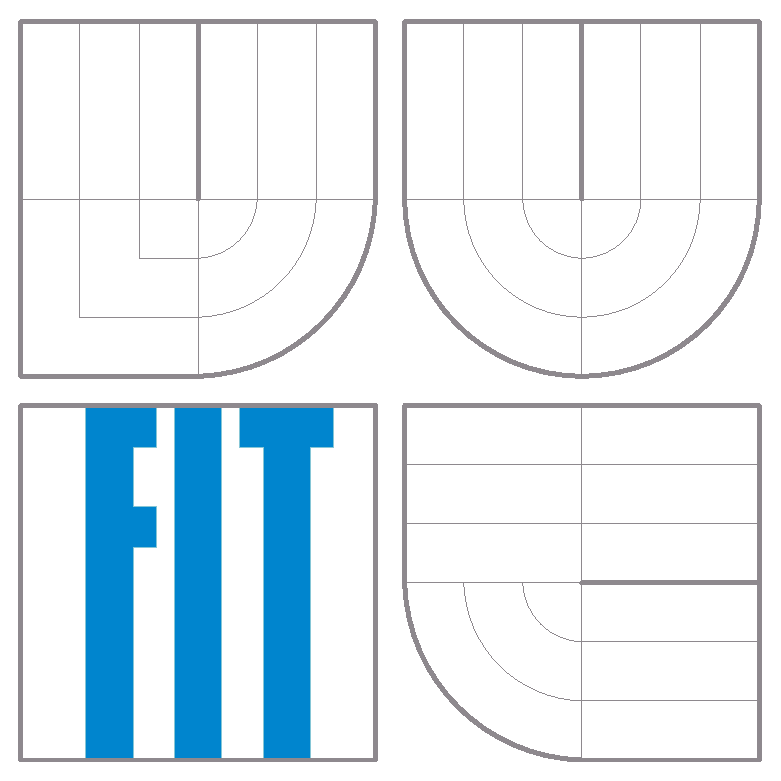
\includegraphics[height=5cm]{images/logo.eps}
	\end{center}
	\vfill
	\begin{center}
		\begin{Large}
			\Course\\
		\end{Large}
		\bigskip
		\begin{Huge}
			\WorkTitle\\
		\end{Huge}
	\end{center}
	\vfill
	\begin{center}
		\begin{large}
			\today
		\end{large}
	\end{center}
	\vfill
	\begin{flushleft}
		\begin{large}
			\begin{tabular}{lll}
				Autor: & \AuthorA, & \url{\AuthorAEmail} \\
				& \AuthorB, & \url{\AuthorBEmail} \\
		
				& & \\
				& \Faculty \\
				& \School \\
			\end{tabular}
		\end{large}
	\end{flushleft}
\end{titlepage}		



% ----- obsah -------------------------------------------------------------
\newpage
\section{Herní enginy}

Jednou z nejpopulárnějších oblastí, zažívající svůj růst v posledních letech kolem WebGL, jsou herní enginy, technologie a různé další frameworky. Výhodou webu jako platformy pro počítačové hry je, že je závislá pouze na internetovém prohlížeči. Nevyžaduje žádné speciální runtimy, není závislá na operačním systému a není třeba nic instalovat. Stačí pouze otevřít prohlížeč, napsat url adresu a hrát. Jedná se tak o řešení vhodná především pro výpočetně jednodušší úkoly a tedy 
hlavně 2D hry.

\subsection{DOM (SVG) a canvas - používané technologie}

\paragraph{DOM} 2D objekty lze ukládat přímo do DOM struktury webové stránky. Využívá se k tomu HTML5 elementů jako \textbf{rect, circle, svg, path}, které jsou ukládány přímo do DOM-u. Při malém množství objektů se jedná o nejrychlejší řešení. Při vyšším se však už zahlcuje DOM a jsou lepší jiná řešení.

\paragraph{Canvas} Další možností pro 2D je využít HTML5 elementu canvas a jeho API. Oproti DOM-u, který se dá považovat za retained mode, se jedná o immediate mode kreslení, kdy nic není ukládáno a vše se rovnou vykresluje pomocí javascriptových metod (např. arc(), fill(), lineTo(),  stroke() atd.). Výhodou je, že se DOM nepřehltí v případě velkého množství objektů. Na druhou stranu vše je vykreslováno v jednom elementu canvas a je tak těžší na jednotlivé objekty vázat nějaké handlery.

\subsection{Srovnání WebGL s Canvas2D a DOM}


\subsubsection{Výhody WebGL}
\begin{itemize}
	\item rychlost u vyššího počtu objektů (10-100x)
	\item více možností - stínovaný, světla, zoom, ...	
	\item hardware akcelerace pro 3D
\end{itemize}
\subsubsection{Nevýhody WebGL}
\begin{itemize}
	\item programovací náročnost - nehodí se na jednoduché aplikace
	\item horší kompatibilita, dnes už pouze Android Browser dělá problémy
\end{itemize}



\begin{figure}[ht]
\begin{center}

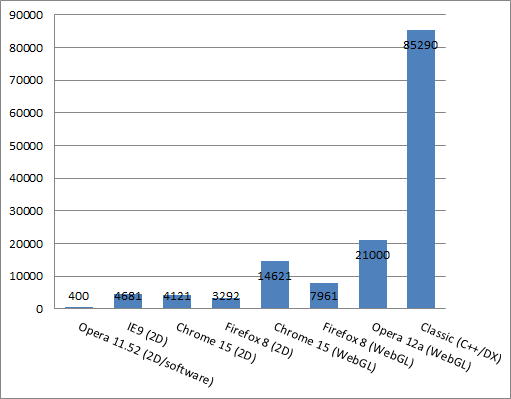
\includegraphics[width=12cm]{images/allperf-graph.png}
\caption{Srovnání vykreslení počtu sprajtů při 30 FPS (Game Engine Construct2) z roku 2011}
\label{fig:theory}
\end{center}
\end{figure}

\newpage

\subsection{Přehled zajímavých knihoven a enginů}

\paragraph{Proč používat jinou knihovnu a ne rovnou WebGL?} Programování ve WebGL je srovnatelné s OpenGL, kdy na vykreslení jednoduché scény s pár krychlemi je třeba stovky řádků kódu - sypete alokujete buffery, sypete do nich bod po bodu, přiřazujete barvu, textury - zkrátka stáráte se o vše a následně. Externí knihovny jako je třeba Three.js umožňují tuto práci výrazně zjednodušit.

Na trhu dnes existuje obrovské množství různých knihoven, především pro tvorbu 2D grafiky. Vybrány jsou perspektivní projekty, které bychom doporučili používat.

\subsubsection{Construct 2}

\url{https://www.scirra.com/construct2}

\begin{itemize}
	\item komerční pro komerční účely, jinak zdarma
	\item 2D herní editor
	\item exportovatelné na platformy: HTML5, Chrome, Facebook, Windows Phone nebo přes wrappery jako CocoonJS na Android či iOS
	\item časově nenáročný vývoj vhodný pro prototypování nebo neprogramátory (není třeba prog. znalostí)
	\item jednoduché hry (Space Invaders, Pac-Man, Tetris, ...)
\end{itemize}

\begin{figure}[ht]
\begin{center}
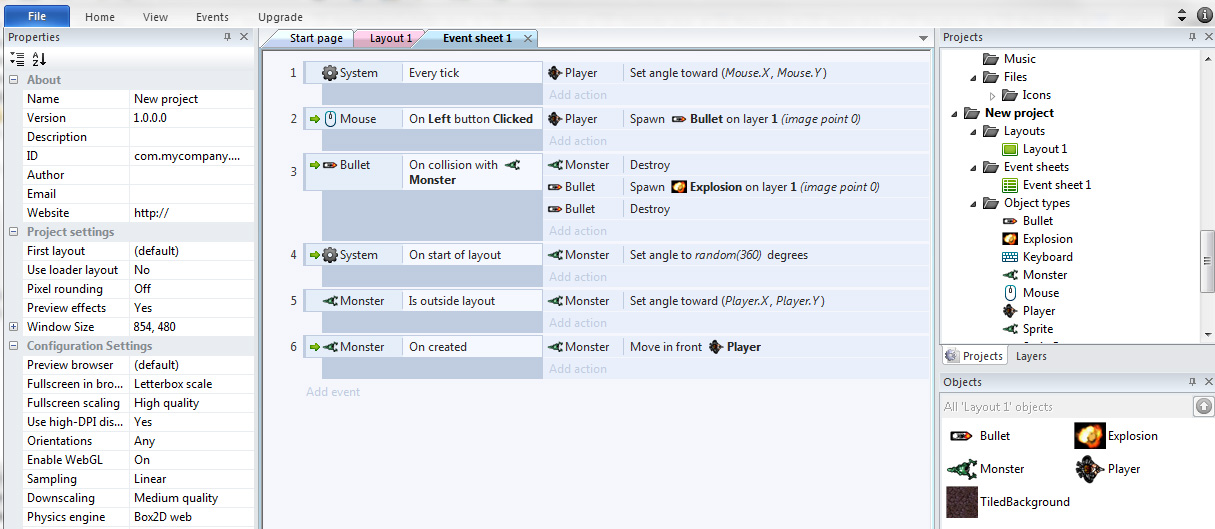
\includegraphics[width=14cm]{images/construct2.jpg}
\caption{Uživatelské rozhraní Construct 2}
\label{fig:theory}
\end{center}
\end{figure}

Při tvorbě aplikace v editoru vytváříte objekty a těm přiřazujete podmínky a následné akce. Nejčastěji se jedná o sprajty, tedy 2D obrázky, ale jako objekty se chovají i vstupní zařízení jako myš nebo klávesnice nebo formulářové prvky. Editor umí pracovata i s AJAXem nebo WebSockets, umožňuje tedy i multiplayer hry a používání databází.

\subsubsection{Three.js}

\url{http://www.threejs.org/}

\begin{itemize}
	\item zdarma (MIT License)
	\item 3D knihovna
	\item Využívá především WebGL, ale pro kompatibilitu umožňuje i Canvas/SVG fallback
	\item Obrovské množství 3D funkcí: materiály, osvětlení, animace, kamera (otrografická, perspektivní), přístup k GLSL, geometrie (plocha, krychle, 3D text, ...), načítání dat (binární, obrázky, přes JSON, ...), matematické funkce a mnohé další	
\end{itemize}

\subsubsection{pixi.js}

\url{http://www.pixijs.com/}

\begin{itemize}
	\item zdarma (MIT License)
	\item 2D knihovna
	\item Scene Graph
	\item WebGL filtry, blending, tinting a další postprocessing efekty
	\item Podpora více dotyků - optimalizováno pro mobilní zařízení
	\item Detekce rendereru - dle podpory zvolí vykreslování pomoci WebGL nebo Canvas2D
	\item Používají i společnosti jako Google nebo McDonalds
\end{itemize}

\subsubsection{Isogenic}

\url{http://www.isogenicengine.com/}

\begin{itemize}
	\item komerční
	\item client-server herní engine specializovaný na multiplayer a masivně hrané multiplayer hry
	\item využívá Node.js, MongoDB, není však náhradou pro HTTP server
	\item mocní síťová komunikace umožnující na jednotlivé klienty streamovat události nebo i celé grafické objekty
	\item jednoduché kreslící funkce (DOM-based nebo Canvas based), nevyužívá WebGL, ale to lze zprostředkovat pomocí jiných knihoven
\end{itemize}

\subsubsection{Závěr}

Každou z předchozích knihoven jsme vyhodnotili jako nejvhodnější pro to co dělá. Pokud máte skvělý nápad a neumíte programovat nebo chcete vytvořit hru za odpoledne, doporučili bychom Construct2. Pro 2D je pak pixi.js, pro 3D naopak three.js. Jako poslední je zmíněn i Isogenic, což je jeden z nejperspektivnějších projektů pro masivně hrané multiplayer hry a lze ho kombinovat i s výše zmíněnými knihovnami.

\subsubsection{Další WebGL herní enginy}
\begin{itemize}
	\item enchant.js (\url{http://enchantjs.com/}) - objektově orientovaný 2D/3D engine japonského původu
	\item PlayCanvas (\url{https://playcanvas.com/}) - 3D engine s editorem, cloud-server a velká komunita, pro nekomerční účely zdarma
	\item Phaser (\url{http://phaser.io/}) - 2D herní engine
	\item voxel.js (\url{http://voxeljs.com/}) - pro milovníky krychlí
\end{itemize}

\subsection{C/C++ - Emscripten - JavaScript}

Za zmínku stojí zmínit i Emscriptem. Jedná se o compiler LLVM kódu do JavaScriptu, především dělaný pro C/C++. Ke kompilaci do LLVM používá Clang, následně LLVM převádí do asm.js nebo JavaScriptu.

\paragraph{Asm.js} \url{http://asmjs.org/} je programovací jazyk tvořený podmnožinou JavaScriptu, přizpůsobený pro výkon ostatních jazyků na webu. Sám o sobě není výkonnější než-li samotný JavaScript - jedná se o jeho podmnožinu, ale při překladu ostatních jazyků s LLVM výstupem do JavaScriptu vykazují tyto jazyky výkonnostní nárůst. Jedná se o projekt Mozilly, Firefox tak byl prvním prohlížečem, který optimalizace asm.js implementoval. Google Chrome je také podporuje.

\begin{figure}[ht]
\begin{center}
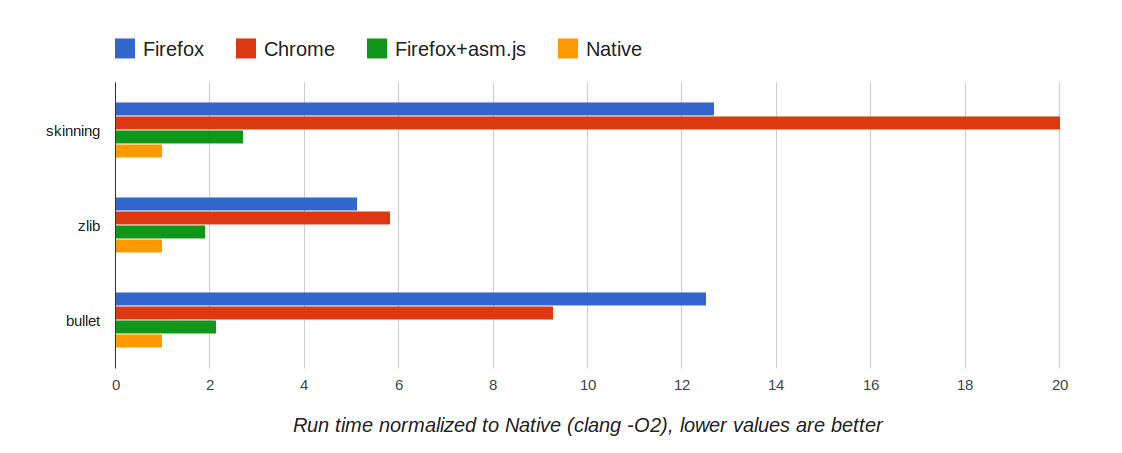
\includegraphics[width=14cm]{images/micro3b.png}
\caption{Srovnání rychlosti nativního kódu a přeloženého kódu}
\label{fig:theory}
\end{center}
\end{figure}

Emscriptem je optimalizován pro překlad OpenGL na WebGL a dobře podporuje i SDL, lze tak převést velké množství aplikací původně napsaných v OpenGL na kód běžící v prohlížeči.

\subsubsection{Zajímavé Emscripten projekty}

Pro nás nejzajímavější je pravděpodobně fakt, že byly již přeloženy projekty založené na herních frameworcích - Unity a Unreal. Součástí Unity5 má být i podpora pro web, která bude pravděpodobně řešena právě tímto přístupem.

\begin{itemize}
	\item DeadTrigger 2 (\url{http://beta.unity3d.com/jonas/DT2/}) - přeložený projekt z Unity
	\item Quake 3 (\url{http://www.quakejs.com/})
	\item Doom (\url{http://kripken.github.io/boon/boon.html})
\end{itemize}

Byly portnuty i aplikace založené na Qt nebo i jiných programovacích jazycích: Ruby, Python, Lua, Perl.

\begin{figure}[ht]
\begin{center}
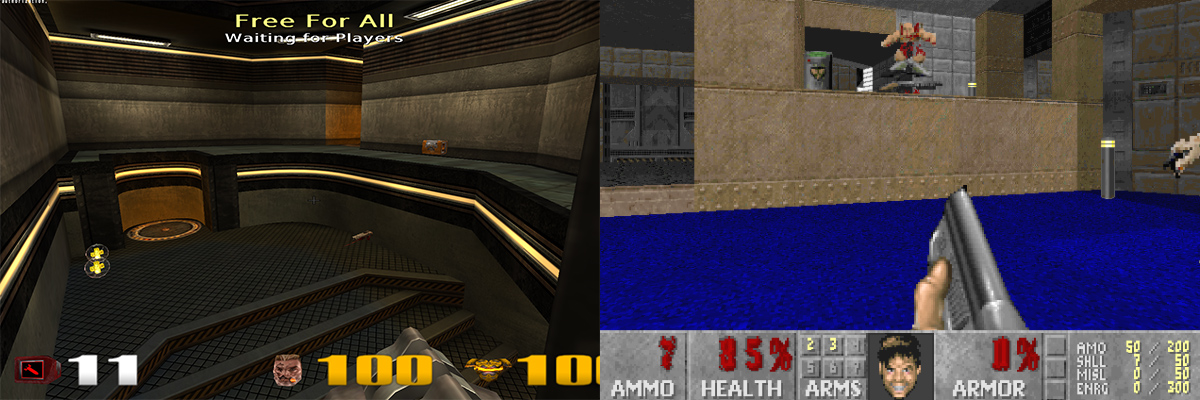
\includegraphics[width=14cm]{images/quakedoom.jpg}
\caption{Příklady portnutých projektů pomocí Emscripten - Quake 3 Arena, Doom}
\label{fig:theory}
\end{center}
\end{figure}

\section{Bezpečnost WebGL a podpora IE}

V roce 2011 Microsoft oznámil, že WebGL nebude podporovat. Tvrdil, že samotné WebGL je nebezpečné jen svým návrhem. Důvody můžou být následující

\begin{itemize}
	\item \textbf{Undefined behaviour} - např. čtení pixelů mimo framebuffer
	\item \textbf{Přístup do nealokované paměti}
	\item \textbf{Shadery} - shadery musí být před předáním grafické kartě validovány
	\item \textbf{DoS} - scéna trvá velkou dobu vykreslit, počítač tak může přestat reagovat
	\item \textbf{Čtení obrázků a videí z cizích zdrojů} - dle specifikace umožněno pouze, pokud je zdroj validován přes CORS (\url{http://www.w3.org/TR/cors/})
\end{itemize}

Výše zmíněné jsou příklady bezpečnostních rizik, které můžou nastat při implementaci v jednotlivých prohlížečích a počítač uživatele tak může být napaden, typicky přestane reagovat.

Asi nejznámějším bezpečnostním problémem WebGL se stalo vykradení grafické paměti uživatele a tím pádem pořízení screenshotů citlivých dat.

S IE11 Microsoft již oznámil, že WebGL podporovat bude. Pravděpodobně pod tlakem konkurence (Firefox, Chrome, Opera), která již technologii dávno podporovala. WebGL v IE11 běží zapouzdřené pod DirectX, což umožňuje v případě, že nastane některá z výše zmíněných bezpečnostních děr, obnovit systém uživatele, v případě, že vypadne.
	

\bibliographystyle{plain}

\nocite{cite1}
\nocite{cite2}
\nocite{cite3}
\nocite{cite4}
\nocite{cite5}
\nocite{cite6}
\nocite{cite7}
\nocite{cite8}
\nocite{cite9}
\nocite{cite10}
\nocite{cite11}
\nocite{cite12}
\nocite{cite13}


\hypertarget{bib}{}
\bibliography{reference}
\addcontentsline{toc}{section}{Literatura}

\end{document}

